\ifpdf
\graphicspath{{Conclusion/Figs/}}
\else
\graphicspath{{Conclusion/Figs/}}
\fi

\chapter*{Conclusion and Research Timeline}
Up till this point, this research has accomplished the following:
\begin{itemize}
	\item Examined the issue of anonymity in Bitcoin and digital currencies
	\item Explored the different ways to anonymise digital currencies and identified Zerocoin as the area of interest
	\item Examined in the detail the Zerocoin protocol and its theoretical basis
	\item Analysed the implementation of Zerocoin and identified areas of improvement
	\item Established the performance metrics and benchmarks to evaluate the proposed improvements 
	\item Proposed an improved Serial Number Signature of Knowledge in Zerocoin Spend transactions and conducted some preliminary tests
	\item Proposed an optimisation for the Accumulator Proof of Knowledge in Zerocoin Spend transactions
\end{itemize}

Going forward, this research plans to work on the following areas:
\begin{itemize}
	\item Set up a peer to peer network that simulates the Zerocoin network to conduct network level tests
	\item Compare the performance of the proposed improvements against the original Zerocoin protocol at the network level
	\item Continue to evaluate the theoretical soundness of the proposed improvements and make necessary adjustments
	\item Further enhance the proposed improvements
	\item Explore ways to improve the other drawbacks in Zerocoin’s functionalities
\end{itemize}

A research timeline outlining the brief schedule for the completed and future tasks is shown in Fig.~\ref{fig:timeline}  

\begin{sidewaysfigure}
	\centering
	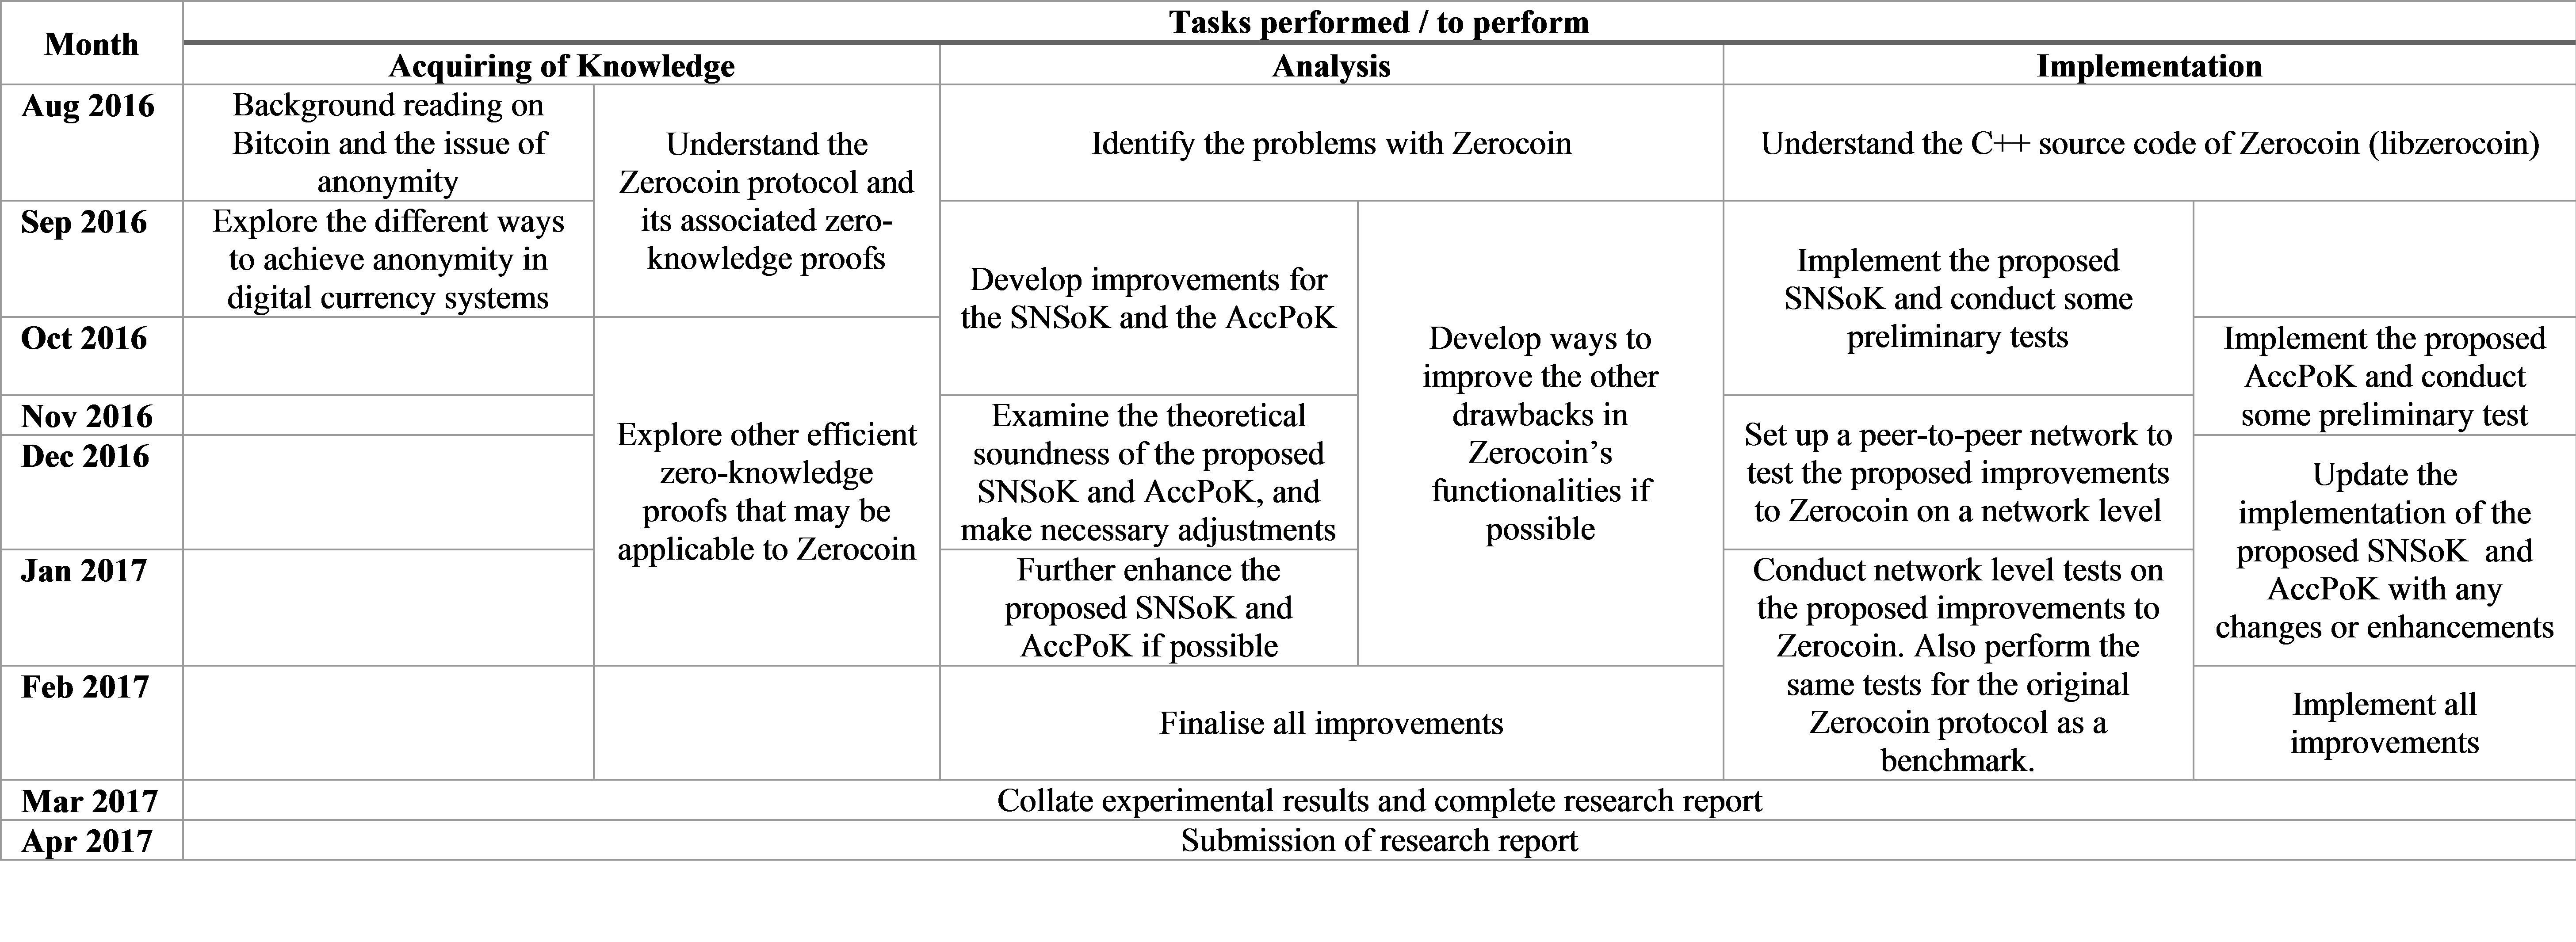
\includegraphics[scale=0.14]{timeline}  
	\caption{Research timeline}
	\label{fig:timeline} 
\end{sidewaysfigure}


